\documentclass[ngerman,pstricks,border=12pt]{standalone}
% --- Pakete einbinden
\input{01_PaketeEinstellungen.tex}
\begin{document}

\begin{figure}[H]
\centering
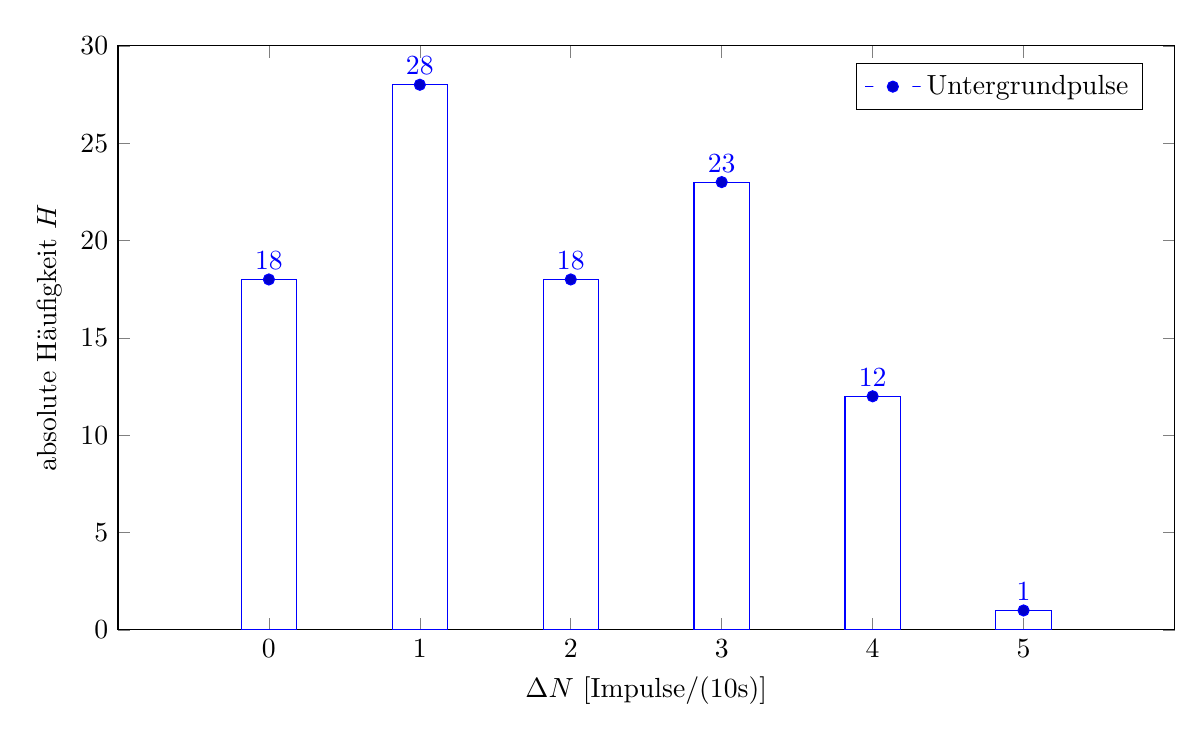
\begin{tikzpicture}
  \begin{axis}[
    width=15 cm,
    height=9 cm,
    xmin=-1, xmax=6,
    ymin=0, ymax=30,
    xlabel={$\Delta N$ [Impulse/(\SI{10}{s})]},
    ylabel={absolute Häufigkeit $H$},
    domain=-3:17,
    legend entries={Untergrundpulse},
    legend pos=north east,
		bar width=20pt,
		xtick={0,1,...,5},
		nodes near coords
  ]
  \addplot+[ybar] plot coordinates {
		(0,18)	(1,28)	(2,18)	(3,23)	(4,12)	(5,1)
		};
  \end{axis}
\end{tikzpicture}
\label{fig:untergrundabsolut}
\end{figure}
\end{document}